\documentclass[12pt]{article}
\usepackage{color,graphicx}
\usepackage{enumitem} %For alphabet bullet points
\usepackage{url} %For proper URL formatting
\usepackage[colorlinks=true, linkcolor=blue, citecolor=blue, urlcolor=blue]{hyperref}
\usepackage{physics}
\usepackage{amsmath} %Might be useful
\usepackage{fancyhdr} % For custom headers and footers

% \newcommand{\Essential}{\href{https://www.google.com/search?q=essential+statistical+physics+kennett+pdf&sca_esv=d12916411115a520&rlz=1C5OZZY_enUS1158US1158&sxsrf=AE3TifN4Zc-ipBPOobbdtRYRqFEYdnWEUw%3A1748901745377&ei=cR8-aI3jFqLGp84PhteR6AY&oq=essential+statistical+physics+ke&gs_lp=Egxnd3Mtd2l6LXNlcnAiIGVzc2VudGlhbCBzdGF0aXN0aWNhbCBwaHlzaWNzIGtlKgIIATIEECMYJzIGEAAYFhgeMgYQABgWGB4yCxAAGIAEGIYDGIoFMgsQABiABBiGAxiKBTILEAAYgAQYhgMYigUyCBAAGIAEGKIEMggQABiABBiiBDIIEAAYgAQYogQyCBAAGIAEGKIESM87UKUdWIUfcAR4AJABAJgBYKABrgGqAQEyuAEDyAEA-AEBmAIGoALFAcICCxAAGIAEGLADGKIEwgIIEAAYsAMY7wWYAwCIBgGQBgWSBwM1LjGgB-oQsgcDMS4xuAe6AcIHBTAuMy4zyAcT&sclient=gws-wiz-serp}{Kennett (2021)}}
% \newcommand{\Thermal}{\href{https://jontalle.web.engr.illinois.edu/Public/BOOKS/Kittel-ThermalPhysics.80.pdf}{Kittel \& Kroemer (1980)}}
% \newcommand{\Intro}{\href{https://perso.crans.org/sylvainrey/Biblio%20Physique/Physique/Thermodynamique/%5BCallen%5D%20Thermodynamics%20and%20an%20Introduction%20to%20Thermostatistics.pdf}{Callen (1985)}}

\textwidth 170mm
\textheight 210mm
\topmargin 0.0mm
\oddsidemargin 0mm
\evensidemargin 0mm
\parindent 0pt

\title{Statistical Mechanics: Qual Review}
\author{Izaiha Martinez \\
The University of Alabama}
\date{\today}

\pagestyle{fancy}
\fancyhf{} % Clear all header and footer fields
\fancyhead[R]{Martinez} % Right side of the header
\fancyfoot[C]{\thepage} % Page number

\pagenumbering{arabic}

\begin{document}

\maketitle

\tableofcontents

\clearpage



\section{Thermaldynamic Laws}

\subsection{0th law}
\begin{itemize}
    \item \textcolor{magenta}{if 2 systems are in equalibrium with a 3rd, they are in equalibrium
    with each other}
\end{itemize}


\subsection{1st law}
\begin{itemize}
    \item \textcolor{magenta}{Conservation of energy}
    \begin{itemize}
        \item assumes condition holds at the microscopic level
    \end{itemize}
    \begin{align}
        dU = dQ + dW
    \end{align}
\end{itemize}


\subsection{2nd law}
\begin{itemize}
    \item \textcolor{magenta}{Entropy always increases}
\end{itemize}


\subsection{3rd law}
\begin{itemize}
    \item \textcolor{magenta}{The entropy per particle goes to zero at absollute zero}
    \begin{itemize}
        \item follows the statistical defintion of enertopy: $S(T = 0) = k_b \ln \Omega_0$
    \end{itemize}
\end{itemize}


\clearpage


\section{Potentials}

\clearpage


\section{Cyclic processes}

\textcolor{violet}{Cyclic processes: thermodynamic process in which a system returns to its initial
	thermodynamic state (i.e same U, P. V. T) after a process.
	\begin{itemize}
		\item aka $\Delta U = 0$
	\end{itemize}
}
\begin{itemize}
	\item We are reminded of the first law: $\Delta U = \Delta Q - p dv$
	      \begin{itemize}
		      \item meaning for a cyclic process  $\rightarrow \Delta U = 0 \rightarrow Q = W$
		      \item total heat added over the cycle = total work done by the system
	      \end{itemize}
	\item Most of this section referenced Chapter 8 (Heat \& Work) from Kittel
\end{itemize}


\subsection{Energy \& Entropy Transfer Definitions}
\begin{itemize}
	\item \textcolor{violet}{heat is the transfer of energy to a system by thermal contact
		      with a reservoir}
	\item \textcolor{violet}{work is the transfer of energy to a system by a change in the
		      external parameters that describe the system}
    \item \textcolor{violet}{entropy transfer in a reversible process is zero when only work is
    performed and no heat is transferred.}
	\item we want to convert heat to work (steam engine, combustion engine)
	\item bringing 2 systems together, the total energy is conserved but not the entropy,
	      may increase
	\item it is defined that $dQ \equiv T dS$ which means $dW = dU - dQ = dU - TdS$
	      \begin{itemize}
		      \item $dS = 0 \rightarrow$ pure work
		      \item $dU = TdS \rightarrow$ pure heat
	      \end{itemize}
\end{itemize}


\subsection{Heat Engines: conversion of heat into work}
\subsubsection{Carnot inequality}
\begin{itemize}
	\item all forms of work are freely convertible, they are thermodynamically
	      equivalent to each other
	\item work can be completely converted to heat but the inverse is not true
	      \begin{itemize}
		      \item entropy enters the system with the heat but does not leave the system with
		            the work
		      \item \textcolor{violet}{"To prevent the accumulation of entropy [in a system] there
			            must be some output heat; therefore it is impossible to convert all the input heat
			            to work!"}
		      \item entropy must ultimately be removed
	      \end{itemize}
	\item heat engine: energy conversion device that operates in cycles
	      \begin{figure}
		      \centering
		      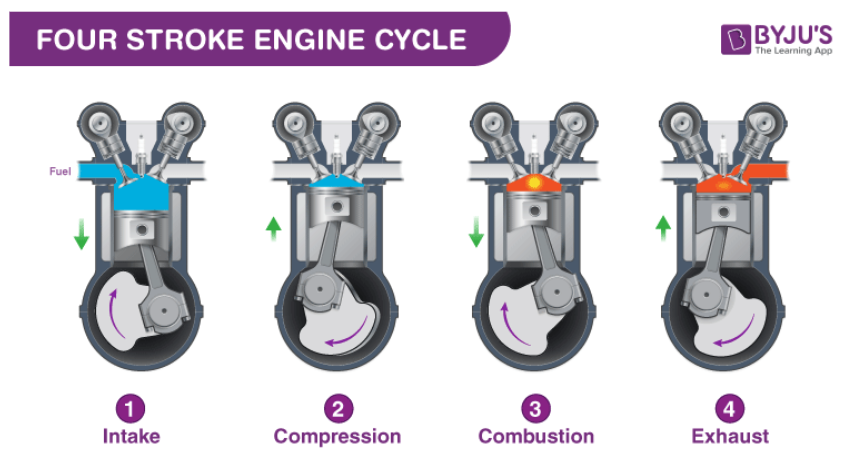
\includegraphics[width=.75\textwidth]{Figures/4StrokeEngineCycle.png}
		      \caption{Entropy is at the min near the beginning of the intake stroke and max at
			      the beginning of the exhaust stroke.}
		      \label{fig:engine_diagram}
	      \end{figure}
	\item work generated during 1 cycle of a reversible process:
	      \begin{align}
		      W = Q_h - Q_l = (1 - T_l/T_h)Q_h = \frac{T_h - T_l}{T_l} Q_h \\
		      \text{Carnot efficiency } \eta_c \equiv (\frac{W}{Q_h})_\text{rev} = \frac{T_h - T_l}{T_l}
	      \end{align}
	      where h is the input heat and l is the leaving heat, \\
	      \textcolor{violet}{aka we can not convert all input heat into work}
	      \begin{align}
		      \text{Carnot inequality } \eta = W/Q \leq 1 - (T_l/T_h) \equiv \eta_c
	      \end{align}
	\item \textcolor{violet}{Carnot inequality is the basic limit for heat engines}
\end{itemize}


\subsubsection{Refrigerators}
\begin{itemize}
	\item refrigerators consume work to remove heat
	      \begin{align}
		      \text{coefficient of refrigerator performance } \lambda \equiv Q_l /W
	      \end{align}
	      $\lambda$ can be greater or less than 1
	      \begin{align}
		      \text{Carnot coefficient of refrigerator performance } \lambda_c = (Q_l/W)_\text{rev} = \frac{T_l}{T_h - T_l}
	      \end{align}
	      \textcolor{violet}{This is an upper limit to the actual coefficient of refrigerator}
	\item air conditioners are refrigerators
	\item heat pumps are reverse connections of an air conditioner
\end{itemize}


\subsubsection{Carnot Cycle}
\begin{itemize}
	\item gas is expanded \& compressed in 4 stages (2 isothermal \& 2 isentropic)
	      \begin{enumerate}
		      \item gas has the temp $T_\text{high}$ \& entropy $S_\text{Low}$
		            \begin{itemize}
			            \item gas expands at constant T until the entropy increases to $S_H$
		            \end{itemize}
		      \item gas has the temp $T_h$ \& entropy $S_H$
		            \begin{itemize}
			            \item gas expands with constant S, until temp drops to $T_l$
		            \end{itemize}
		      \item gas has the temp $T_l$ \& entropy $S_H$
		            \begin{itemize}
			            \item gas is compressed isothermally
		            \end{itemize}
		      \item gas has the temp $T_l$ \& entropy $S_L$
		            \begin{itemize}
			            \item compressed isentropically to original state
		            \end{itemize}
	      \end{enumerate}
	\item work done by the system is the area of the rectangle (Carnot cycle)
	      \begin{align}
		      W & = (T_h - T_l) (S_H - S_L) \\
	      \end{align}
	      which comes from
	      \begin{align}
		      \oint dU = 0 = \oint TdS - \oint pdV \rightarrow W = \oint TdS
	      \end{align}
\end{itemize}


\subsubsection{Path Dependence of Heat \& Work}
\begin{itemize}
	\item transfers of heat and work between state (a) and state (b) depend on the path
	      taken between the two states \textcolor{violet}{heat \& work are not state functions}
	\item "Without the path dependence of heat and work there would not exist cyclical
	      processes that permit the generation of work from heat."
\end{itemize}

\subsubsection{Irreversible Work}
\begin{itemize}
	\item if newly created entropy arises by the conversion of work to heat, irreversible
	      work has been performed
	\item pure heat transfer not involving any work done between 2 systems with different temperatures
\end{itemize}


\subsection{Heat \& Work at Constant Temp or Pressure}

\begin{itemize}
    \item Isobaric process: constant pressure
    \item the effective work $dW \equiv dW + d(pV) = dU + d(pV) -dQ = dH - dQ$
    where H is enthalpy ($H = U + pV$)
    \begin{itemize}
        \item $dQ = dH$: no effective work is done (heat liquid with no cap)
        \item constant pressure and temp $dQ = T dS = d(TS)$
    \end{itemize}
    \item \textcolor{violet}{use enthalpy at constant pressure}
    \item \textcolor{violet}{use gibbs free energy at constant P \& T} ($G = F + pV = U +pV - TS$)
\end{itemize}

\subsubsection{Chemical Work}
\begin{itemize}
    \item Chemical work: work performed by the transfer of particles to a system (associated with
    chemical potential)
    \begin{align}
        dW = \mu dN
    \end{align}
    \item Chemical potential (reference figure 8.14)
    \begin{itemize}
        \item is the work required to transfer 1 particle into the system
        \item the difference in chemical potential between 2 systems is equal to the net work
        required to move a particle from 1 system to the other (if there is 0 volume work)
        $dW = \mu_a dN_a + \mu_b dN_b = (\mu_b - \mu_a)dN$
        \begin{figure}[h]
            \centering
            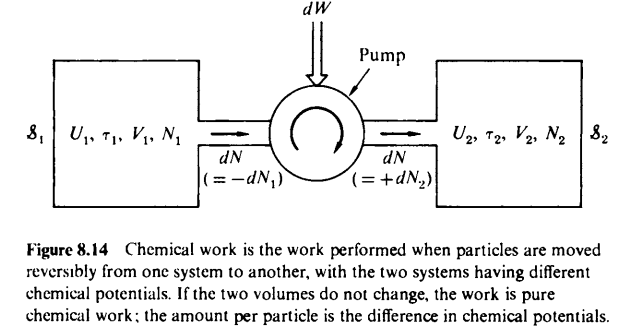
\includegraphics[width=.75\textwidth]{Figures/chemical_work.png}
            \label{fig:chemical_work}
        \end{figure}
        \item if 2 systems are in diffuse equilibrium ($\mu_a = \mu_b$), no work is required to move
        the particles
    \end{itemize}
\end{itemize}


\subsubsection{Heat Capacity}
\begin{itemize}
    \item the heat capacity is the amount of heat needed to raise its temperature per degree
    \begin{align}
        C \equiv \frac{Q}{\Delta T} = \frac{\Delta U + p dv}{\Delta T}
    \end{align}
    \item where the specific heat capacity is simply the heat capacity per unit of mass ($c \equiv \frac{C}{m}$)
    \item Where we can take a case of constant volume (no work is done) and use the thermodynamic
    identity to get
    \begin{align}
        C_V = \frac{\Delta U + 0}{\Delta T}|_V = \pdv{U}{T}|_V
    \end{align}
    which we can also substitute back $dq$ as we know $dq = T dS$:
    \begin{align}
        C_V = \pdv{U}{T}|_V = T \pdv{S}{T}|_V
    \end{align}
    \item for the case where we have constant P we have
    \begin{align}
        C_P = \frac{\Delta U + pdv}{\Delta T}|_P = \frac{\Delta U}{\Delta T}|_P + p \frac{\Delta V}{\Delta T}|_P
    \end{align}
	\item molar heat capacity, simply the heat capacity per mole of atoms
	\begin{align}
		c_m = \frac{C}{n}
	\end{align}
	\item thermal expansion coefficient: materials expand when they are heated, this coefficient is the fractional
	increase in volume per unit change in temperature
	\begin{align}
		\beta \equiv \frac{\Delta V/V}{\Delta T}
	\end{align}
	\item linear thermal expansion coefficient:
	\begin{align}
		\alpha \equiv \frac{\Delta L /L}{\Delta T}
	\end{align}
	\item isothermal compressibility
	\begin{align}
		\kappa_T \equiv -\frac{1}{V} \pdv{V}{P}|_T
	\end{align}
\end{itemize}

\subsection{Latent Heat}
\begin{itemize}
	\item how much heat is required to melt or boil a substance, the amount divided by the mass of the substance
	\begin{align}
		L \equiv \frac{Q}{m}
	\end{align}
\end{itemize}

\subsection{Some Discussion Notes}
\begin{itemize}
	\item reversible process
	      \begin{itemize}
		      \item to begin this system has no change in energy as well as entropy (like wut???)
		      \item since there is no change in entropy, it stands that there is no change in temp as:
		            \begin{align}
			            \Delta S_\text{tot} = \frac{-Q}{T_A} + \frac{Q}{T_B}
		            \end{align}
		            which means that there is no heat exchange
		      \item since $\Delta U = 0$ \& $\Delta Q = 0$ it stands that $\Delta W = 0$
		            ($\Delta U = \Delta Q - \Delta W$), \textcolor{violet}{aka no work is done!!}
		      \item this system is also quassi static which means it's always in equilibrium
	      \end{itemize}
\end{itemize}


\subsection{Example Problems to try:}
\begin{itemize}
    \item 2024 Qual: \#1, \#3, \#4
\end{itemize}


\clearpage


\section{Equilibrium Ensembles I.}

\subsection{Micro-canonical}

\subsection{Canonical}

\subsection{Grand-canonical}


\clearpage

\section{Equilibrium Ensembles II.}

\subsection{Classical Cases}

\subsection{Quantum Cases}


\clearpage

\section{Ideal Quantum Gases \& Applications}


\clearpage



\section{Equation Sheet}

\subsection*{Forms of Entropy:}

\begin{align}
	S(N, U) = k \log \Omega
\end{align}

\subsection*{Partial derivatives:}

\begin{align}
	\text{Entropy: } S(U, N, V) =
	\begin{cases}
		\pdv{S}{U} = \frac{1}{T}    \\
		\pdv{S}{V} = \frac{P}{T}    \\
		\pdv{S}{N} = -\frac{\mu}{T} \\
	\end{cases}
\end{align}

\subsubsection*{\textcolor{magenta}{Maxwell's Relation:}}

\begin{align}
	\text{Energy: }                & U(S, V, N) = TS - PV + \mu N
	\begin{cases}
		\pdv{U}{S} = T   \\
		\pdv{U}{V} = -P  \\
		\pdv{U}{N} = \mu \\
	\end{cases}                                               \\
	\text{Helmholts Free Energy: } & F(T, N, V) = U - T S(U, N, V)
	\begin{cases}
		\pdv{F}{T} = -S  \\
		\pdv{F}{N} = \mu \\
		\pdv{F}{V} = -P  \\
	\end{cases}                                               \\
	\text{Gibbs Free Energy: }     & G(N, T, P) = F(N, T, V) + PV
	\begin{cases}
		\pdv{G}{T} = -S  \\
		\pdv{G}{P} = V   \\
		\pdv{G}{N} = \mu \\
	\end{cases}                                               \\
\end{align}

\subsubsection*{Other Partial Derivatives:}

\begin{align}
	\text{Enthalpy: }       & H(S, P, N) = U + PV
	\begin{cases}
		\pdv{H}{S} = T   \\
		\pdv{H}{P} = V   \\
		\pdv{H}{N} = \mu \\
	\end{cases}                                               \\
	\text{Grand Potential:} & \Phi(T, \mu, V) = \mu N - F(T, N, V)
	\begin{cases}
		\pdv{\Phi}{T} = S   \\
		\pdv{\Phi}{\mu} = N \\
		\pdv{\Phi}{V} = P   \\
	\end{cases}
\end{align}

\subsection*{Ideal Gas:}
\begin{align}
	PV & = NKT = nRT                                                 \\
	U  & = \frac{f}{2} KT \text{, where f is the degrees of freedom}
\end{align}

\subsection*{Partition Function:}

\begin{align}
	\text{Normal:  } z & = \sum e^{E_i / kT}                                                                                            \\
	\text{One: } z_1   & = \frac{1}{h^3} \int d^3x d^3p e^{-E/ kT}\text{, where } d^3 = p^2\sin\theta dp d\theta d\phi                  \\
	\text{Many: } z_N  & = \frac{1}{N!} z_1^N                                                                                           \\
	\text{Grand: } \Xi & = \sum_{N=0}^{\inf} z_N e^{\mu N / kT} = \sum_{N=0}^{\inf} \frac{1}{N!} (\sum_a e^{E_a / kT})^N e^{\mu N / kT}
\end{align}


\subsection*{Free Energy Forms:}
\begin{align}
	F = - KT \ln(z)
\end{align}

\subsection*{Heat}
\begin{align}
	dS & = \frac{dQ}{T} \\
	S  & = \frac{Q}{T}
\end{align}

\subsubsection*{In a Carnot Cycle}
\begin{align}
	\oint dU = 0 = \oint TdS - \oint pdV \rightarrow W = (T_h - T_l) (S_H - S_L)
\end{align}

\subsection*{A Thermodynamic Identity}
\begin{align}
	dU = TdS -pdV \rightarrow	TdS = dU + p dV
\end{align}

\subsection*{To cover all bases equations:}
\begin{align}
	\text{Pressure } P               & = \rho g h                                                \\
	\text{Force } F                  & = P * A = \rho g V                                        \\
	\text{Carnot efficiency } \eta_c & \equiv (\frac{W}{Q_h})_\text{rev} = \frac{T_h - T_l}{T_l}
\end{align}

\subsection*{Approximations}

\begin{itemize}
	\item Stirling Approximation (large limits of n ignore the $O$ term)
	      \begin{align*}
		      \ln(n!) & = n \ln(n) - n + O(\ln(n)) \\
		      \ln(n!) & \approx n \ln(n) - n
	      \end{align*}
\end{itemize}


\subsection*{Dumb Abbreviations}
\begin{align*}
	k T    & = \tau  = \beta^{-1} \\
	\sigma & = \log g             \\
	S      & = k \sigma
\end{align*}






\end{document}
